%! Author = amatarazzo
%! Date = 09/05/24

\chapter{Utilization Strategies and Techniques}
\label{ch:utilization}

\section{Introduction}
\label{sec:ch4-introduction}

In this chapter, we will discuss the strategies and techniques that can be used to utilize large language models effectively.
We will start by discussing the importance of context in utilizing large language models and how it can be used to improve their performance.
We will then move on to the concept of chain-of-thought prompting and how it can be used to guide the generation of text.
Finally, we will discuss the importance of planning for complex tasks and how it can be used to improve the performance of large language models.

\begin{table}[h!]
	\centering
	\tiny
	\begin{tabularx}{\textwidth}{|l|X|X|}
		\hline
		\textbf{Approach}                         & \textbf{Representative Work}                                                                                                                                                                                                                                                                                                                                                                                                                 & \textbf{Key Point}                                                                                                                                                                                                                                                                                                                                                                                                                                                                                                                                                                                                                                                                                                                                                                                                                                                          \\
		\hline
		\textbf{In-context Learning (ICL)}        & KATE~\cite{liu2022good}, EPR~\cite{rubin2022learning}, SG-ICL~\cite{kim2022self}, APE~\cite{zhou2023large}, Structured Prompting~\cite{hao2022structured}, GlobalE \& LocalE~\cite{lu2022fantastically}                                                                                                                                                                                                                                      & Demonstration selection (similar, k-NN) \newline Demonstration selection (dense retrieval; contrastive learning) \newline Demonstration selection (LLM as the demonstration generator) \newline Demonstration format (automatic generation \& selection) \newline Demonstration format (grouped context encoding; rescaled attention) \newline Demonstration order (entropy-based metric; probing set generation with LLM)                                                                                                                                                                                                                                                                                                                                                                                                                                                  \\
		\hline
		\textbf{Chain-of-thought Prompting (CoT)} & Complex CoT~\cite{fu2022complexity}, Auto-CoT~\cite{zhang2022automatic}, Selection-Inference~\cite{creswell2022selection}, Self-consistency~\cite{wang2022self}, DIVERSE~\cite{li2022advance}, Rationale-augmented ensembles~\cite{wang2022rationale}                                                                                                                                                                                        & Demonstration (complexity-based selection) \newline Demonstration (automatic generation) \newline Generation (alternate between selection and inference) \newline Generation (diverse paths; self-ensemble) \newline Generation (diverse paths; Verification (step-wise voting)) \newline Generation (rationale sampling)                                                                                                                                                                                                                                                                                                                                                                                                                                                                                                                                                   \\
		\hline
		\textbf{Planning}                         & Least-to-most prompting~\cite{zhou2022least}, DECOMP~\cite{khot2022decomposed}, PS~\cite{wang2023plan}, Faithful CoT~\cite{lyu2023faithful}, PAL~\cite{gao2022pal}, HuggingGPT~\cite{shen2023hugginggpt}, AdaPlanner~\cite{sun2023adaplanner}, TIP~\cite{lu2023multimodal}, RAP~\cite{hao2023reasoning}, ChatCoT~\cite{chen2023chatcot}, ReAct~\cite{yao2022react}, Reflexion~\cite{shinn2023reflexion}, Tree of Thoughts~\cite{yao2023tree} & Plan generation (text-based; problem decomposition) \newline Plan generation (text-based; problem decomposition) \newline Plan generation (text-based) \newline Plan generation (code-based) \newline Plan generation (code-based; Python) \newline Plan generation (code-based; models from HuggingFace) \newline Plan refinement (skill memory) \newline Feedback acquisition (visual perception) \newline Feedback acquisition (LLM as the world model; Plan refinement (Monte Carlo Tree Search)) \newline Feedback acquisition (tool); Plan refinement (conversation between LLM and tools) \newline Feedback acquisition (tool); Plan refinement (synergizing reasoning and acting) \newline Feedback acquisition (text-based self-reflection); Plan refinement (dynamic memory) \newline Feedback acquisition (vote comparison); Plan refinement (tree-based search) \\
		\hline
	\end{tabularx}
	\caption{Typical LLM utilization methods and their key points for ICL, CoT, and planning. Note that the key points only highlight the most important technical contribution. Source: \textcite{survey}}
	\label{tab:utilization-methods}
\end{table}

\section{In-Context Learning}
\label{sec:in-context-learning}
In-context learning is a special prompting technique, initially introduced by \textcite{brown2020language}, that allows the model to learn from the context of the prompt (examples shown in Figure~\ref{fig:in-context-learning}).
\begin{figure}[h!]
	\centering
	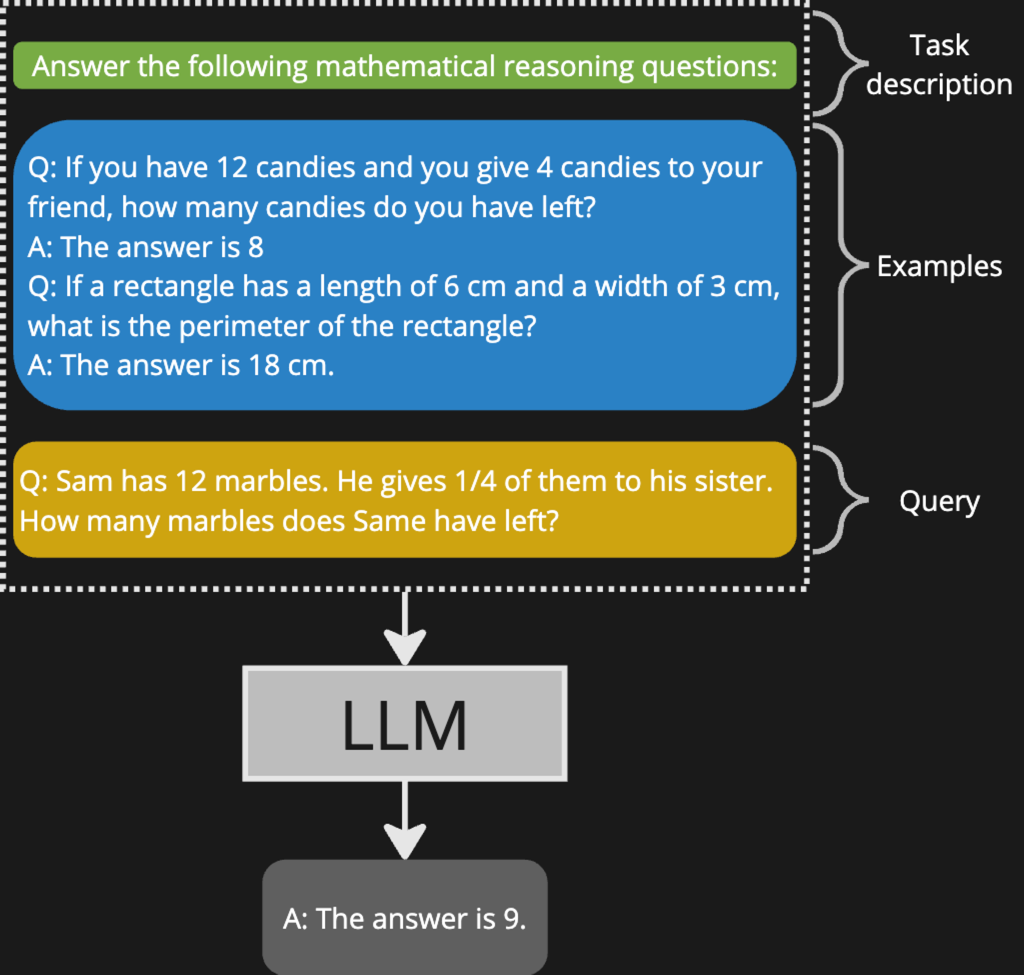
\includegraphics[width=\textwidth]{icl}
	\caption{In-context learning contrasted with traditional fine-tuning. Source: \textcite{brown2020language}}
	\label{fig:in-context-learning}
\end{figure}
ICT consists of the task description and/or few examples of the task as demonstrations combined in a specific order to form natural language prompts with specifically designed templates~\cite{brown2020language}.
Finally, the test instance is appended to the prompt to form the input for LLMs to generate the output.

Based on task demonstrations, LLMs can learn to perform a new task without explicit gradient update.
Formally, the in-context learning task can be defined as follows:
\begin{equation}
	LLM(I, \underbrace{f(x_1, y_1), \dots, f(x_k, y_k)}_\text{demonstrations}, \underbrace{f(x_{k+1}}_\text{input}, \underbrace{\uline{~~~}}_\text{answer})) \rightarrow \hat{y}_{k+1}
	\label{eq:ict}
\end{equation}
where $I$ is a task description, $f(x_i, y_i)$ function that convert task demonstration to natural language, $x_{k+1}$ is a new input query, $\hat{y}_{k+1}$ is the prediction of the output generated, and the actual answer $y_{k+1}$ is left as a blank to be predicted by the LLM\@.

\begin{figure}[h!]
	\centering
	\resizebox{\textwidth}{!}{
		\begin{forest}
			forked edges,
			for tree={
					grow=east,
					reversed=true, % reverse the direction of growth
					anchor=base west, % align text to the west
					parent anchor=east,
					child anchor=west,
					base=left,
					font=\small,
					rectangle,
					draw,
					align=left,
					s sep=3mm, % sibling distance
					l sep=10mm, % level distance
					inner xsep=3mm, % text padding horizontal
					inner ysep=1mm  % text padding vertical
				}
				[In-context Learning
						[Inference
								[Scoring Function
										[{Channel prompt tuning~\cite{min2022metaicl},\\
													kNN-Prompting~\cite{xu2023knn}}]
								]
								[Demonstration Designing
										[Organization
												[Selecting
														[{KATE~\cite{liu2022good}, \\
																	EPR~\cite{rubin2022learning}, \\
																	PPL~\cite{gonen2022demystifying}, \\
																	SG-ICL~\cite{kim2022selfgenerated}, \\
																	Self Adaptive~\cite{wu2022selfadaptive}, \\
																	MI~\cite{sorensen2022information}, \\
																	Q-Learning~\cite{zhang2022active}, \\
																	Informative Score~\cite{li2023finding}, \\
																	Topic~\cite{wang2023large}, \\
																	UDR~\cite{li2023finding}}]
												]
												[Ordering
														[{GlobalE\&LocalE~\cite{lu2022fantastically}}]
												]
										]
										[Formatting
												[Instruction
														[{Instruction Induction~\cite{honovich2022instruction}, \\
																	APE~\cite{zhou2022least}, \\
																	Self-Instruct~\cite{wang2022selfinstruct}}]
												]
												[Reasoning Steps
														[{CoT~\cite{wang2022selfinstruct}, \\
																	Complex CoT~\cite{fu2022complexity}, \\
																	AutoCoT~\cite{zhang2022automatic}, \\
																	Self-Ask~\cite{press2022train}, \\
																	MoT~\cite{li2023mot}, \\
																	SuperICL~\cite{xu2023small}, \\
																	iCAP~\cite{wang2022iteratively}, \\
																	Least-to-Most Prompting~\cite{zhou2022least} }]
												]
										]
								]
						]
						[Training
								[Warmup
										[Self-supervised In-context Training
												[{Self-supervised ICL~\cite{chen2022improving}, \\
															PICL~\cite{gu2023pretraining}}]
										]
										[Supervised In-context Training
												[{MetaICL~\cite{min2022metaicl}, \\
															OPT-IML~\cite{iyer2022opt}, \\
															FLAN~\cite{wei2022fine}, \\
															Super-NaturalInstructions~\cite{wang2022super}, \\
															Scaling Instruction~\cite{chung2022scaling}, \\
															Symbol Tuning~\cite{wei2023symbol}}]
										]
								]
						]
				]
		\end{forest}
	}
	\caption{Taxonomy of in-context learning. The training and the inference stage are two main stages for ICL. During the training stage, existing ICL studies mainly take a pretrained LLM as backbone, and optionally warmup the model to strengthen and generalize the ICL ability. Towards the inference stage, the demonstration designing and the scoring function selecting are crucial for the ultimate performance. Source: \textcite{dong2023survey}}
	\label{fig:icl-taxonomy}
\end{figure}

Since the performance of ICL heavily relies on demonstrations, it is important to properly design them in the prompts.
The tree main aspects are a direct consequence of what defined in the the Equation~\ref{eq:ict}: how to select the task demonstrations, how to convert them into natural language, and arrange demonstrations in a reasonable order.

Different training strategies enhance ICL capabilities, improving performance across various tasks without specific task optimization during the pre-training phase (see Figure~\ref{fig:icl-taxonomy} under the Training branch).
Main approaches include Supervised In-context Training, such as MetaICL\footnote{Meta-training for InContext Learning} and Symbol Tuning, and Self-supervised In-context Training, such as Self-supervised ICL and PICL~\cite{dong2023survey}.

MetaICL~\cite{min2022metaicl} proposed to continually train LLMs on a wide range of tasks\footnote{Classification, question answering,
	natural language inference, paraphrase detection and more} with demonstration examples.
This approach is related to other works that uses multi-task learning for better zero-shot performance at test time~\cite{min2022metaicl}.
However, MetaICL is distinct as it allows learning new tasks from k examples alone, without relying on a task reformatting (e.g., reducing everything to question answering)
or task-specific templates (e.g., converting different tasks to a language modeling problem).
MetaICL is based on the core idea of in-context learning by conditioning on training examples (i.e., explicitly training on an in-context learning objective).

Symbol Tuning~\cite{wei2023symbol} instead fine-tunes language models on in-context input-label pairs, substituting natural language labels (e.g., "positive/negative sentiment") with arbitrary symbols (e.g., "foo/bar").
As a result, symbol tuning demonstrates an enhanced capacity to utilize in-context information for overriding prior semantic knowledge.
Compared to MetaICL, which constructs several demonstration examples for each task, instruction tuning mainly considers an explanation of the task and is more easier to scale up.

Self-supervised ICL leverages raw corpora to generate input/output pairs as training data, while PICL also utilizes raw corpora but employs a simple language modeling objective, promoting task inference and execution based on context.
PICL shown to be more effective in zero-shot settings and tasks generalization~\cite{dong2023survey}.

Effective demonstration design is crucial, involving selecting and ordering examples, or using instruction induction and reasoning steps (as shown in Figure~\ref{fig:icl-taxonomy} under the Inference/ Demonstration Designing branch).
The selection aims to choose good examples for ICL using unsupervised\footnote{Based on pre-defined metrics} or supervised methods.
For example, KATE~\cite{liu2022good} and EPR~\cite{rubin2022learning} select demonstrations based on similarity.
The ordering of the selected demonstrations is also an important aspect of demonstration design.
\textcite{lu2022fantastically} have proven that order sensitivity is a common problem and affects various models.
To handle this problem, studies have proposed several training-free methods to order demonstrations.
\textcite{liu2022good} sorted examples based on similarity, while GlobalE\&LocalE~\cite{lu2022fantastically} orders demonstrations based on global and local entropy.

A common representation of demonstrations is concatenating examples $(x_1, y_1), \cdots, (x_k, y_k)$ with a template T directly.
However, this approach may not be optimal for all tasks, i.e.\ when the task is complex or requires multiple steps such as math word problems and common-sense reasoning.
In those cases, it's not easy to learn the mapping from $x_i$ to $y_i$ with only $k$ demonstrations.
Template engineering has been studied in \textcite{liu2021pretrain, liu2022good} to generate task-specific templates.
Some researches have proposed to design a better format of demonstrations, by describing tasks with instructions I and adding intermediate reasoning steps between examples $(x_i, y_i)$.
Instructions depends heavily on human input, but they can be generated automatically as shown in \textcite{honovich2022instruction} given several demonstration examples.
\textcite{zhou2023large} proposed APE for automatic instruction generation and selection.
To further improve the quality of the automatically generated instructions, \textcite{wang2022selfinstruct} proposed Self-Instruct, which is able to get rid of its own generations.

The approach of adding intermediate reasoning steps between examples introduced in \textcite{wang2023large} is also called Chain-of-Thought prompting.
We will delve into Chain-of-Thought prompting in the next Section~\ref{sec:chain-of-thought}.

At the inference stage, ICL operates without explicit updates, focusing on task recognition and learning through demonstrations.
Task recognition utilizes pre-trained knowledge to solve tasks identified in the demonstrations.
A Probably Approximately Correct (PAC)~\cite{wies2023learnability} framework has been proposed to evaluate ICL’s learnability, suggesting that LLMs can recognize tasks from minimal inputs.

Task learning, on the other hand, involves LLMs learning new tasks through demonstrations, akin to implicit fine-tuning through the attention mechanism, which generates meta-gradients.
With the examples provided in ICL, LLMs can implement learning algorithms such as gradient descent or directly compute the closed-form solution to update these models during forward computation.
Under this explanation framework, it has been shown that LLMs can effectively learn simple linear functions and even some complex functions like decision trees with ICL~\cite{akyurek2022what}.
Different model scales exhibit distinct capabilities; smaller models are adept at task recognition, while larger models (at least 66 billion parameters) are necessary for task learning~\cite{pan2023what}.

\begin{table}[h!]
	\centering
	\small
	\begin{tabularx}{0.8\textwidth}{lXccc}
		\toprule
		\textbf{Scoring Function} & \textbf{Target}              & \textbf{Efficiency} & \textbf{Task Coverage} & \textbf{Stability} \\
		\midrule
		Direct                    & $\mathcal{M}(y_j \mid C, x)$ & +++                 & +                      & +                  \\
		PPL                       & PPL($S_j$)                   & +                   & +++                    & +                  \\
		Channel                   & $\mathcal{M}(x \mid C, y_j)$ & +                   & +                      & ++                 \\
		\bottomrule
	\end{tabularx}
	\caption{Summary of different scoring functions.}
	\label{tab:scoring-functions}
\end{table}

The last piece of ICL is the scoring function, which decides how to transform the predictions of the LLMs into an estimation of the likelihood of a specific answer.
A direct estimation method adopts the conditional probability of candidate answers and select the higher probability as the final answer~\cite{brown2020language}.
However, this method poses some restrictions on the template design, e.g., the answer tokens should be placed at the end of input sequences.
Perplexity (PPL) is another commonly-used metric that computes the PPL of the entire input sequence:
\begin{equation}
	S_j = \{C,s(x,y_i,I)\}
	\label{eq:ppl}
\end{equation}
where C are the tokens of the demonstration examples, $x$ is the input query, and $y_i$ is the candidate label.
As PPL is a global metric (i.e., it considers the entire input sequence), it removes the limitations of token positions but requires extra computation time.
In generation tasks such as machine translation, ICL predicts the answer by decoding tokens with the highest sentence probability combined with diversity-promoting strategies such as beam search or Top-p and Top-k~\cite{holzman2020curious} sampling algorithms.
\textcite{min2022noisy} proposed a channel scoring function that estimates the likelihood of the input query given the candidate answer\footnote{Compute the conditional
	probability in a reversed direction}, which is more efficient and stable than the direct estimation method.
In this way language models are required to generate every token in the input, which could boost the performance under imbalanced training data regimes.
To calibrate the bias or mitigate the sensitivity via scoring strategies some studies add additional calibration parameters to adjust the model predictions~\cite{zhao2021calibrate}.

\subsection{ICL performance and origins}
\label{subsec:icl-performance}

Knowing and understanding the factors that influence ICL can help to improve the performance of LLMs.
ICL has a close connection with instruction tuning (discussed in Section~\ref{subsec:instruction-tuning}) in that both utilize natural language to format the task or instances.
However, instruction tuning needs to fine-tune LLMs for adaptation, while ICL only prompts LLMs for utilization~\cite{survey}.
Furthermore, instruction tuning can enhance the ICL ability of LLMs to perform target tasks, especially in the zero-shot setting\footnote{Using only task descriptions}~\cite{chung2022scaling}.

\begin{table}[h!]
	\centering
	\small
	\begin{tabularx}{0.8\textwidth}{lX}
		\toprule
		\textbf{Stage} & \textbf{Factor}                                                                               \\
		\midrule
		\multirow{4}{*}{Pretraining}
		               & Pretraining corpus domain~\cite{shin2022effect}                                               \\
		               & Pretraining corpus combination~\cite{shin2022effect}                                          \\
		               & Number of model parameters~\cite{wei2022emergent, brown2020language}                          \\
		               & Number of pretraining steps~\cite{wei2022emergent}                                            \\
		\midrule
		\multirow{8}{*}{Inference}
		               & Label space exposure~\cite{min2022rethinking}                                                 \\
		               & Demonstration input distribution~\cite{min2022rethinking}                                     \\
		               & Format of input-label pairing~\cite{min2022rethinking,an2023how}                              \\
		               & Demonstration input-label mapping~\cite{min2022rethinking, yoo2022groundtruth, wei2023symbol} \\
		               & Demonstration sample ordering~\cite{lu2022fantastically}                                      \\
		               & Demonstration-query similarity~\cite{lu2022fantastically}                                     \\
		               & Demonstration diversity~\cite{an2023how}                                                      \\
		               & Demonstration complexity~\cite{an2023how}                                                     \\
		\bottomrule
	\end{tabularx}
	\caption{Summary of factors that have a relatively strong correlation to ICL performance. Source: \textcite{dong2023survey}}
	\label{tab:icl-factors}
\end{table}

There are several factors that have a relatively strong correlation to ICL performance, as shown in Table~\ref{tab:icl-factors}.
ICL ability may give raise putting multiple corpora together in the pre-training stage, and the domain source is more important than the corpus size~\cite{shin2022effect}, while pretrain on corpora related to downstream tasks and models with lower perplexity do not always perform better in ICL~\cite{shin2022effect}.
\textcite{wei2022emergent} suggested that a pretrained model suddenly acquires some emergent ICL abilities when it achieves a large scale of pretraining steps or model parameters and \textcite{brown2020language} showed that the ICL ability grows as the parameters of LLMs increase from 0.1 billion to 175 billion.
At inference stage, the properties of the demonstrations influence the ICL performance, such as the label space exposure, the format of input-label pairing, the ordering of demonstration samples, and the complexity of demonstrations~\cite{min2022rethinking, an2023how, lu2022fantastically}.
There are contrasting results on the impact of input-label mapping related to ICL~\cite{min2022rethinking, yoo2022groundtruth}.
An interesting finding is that, when a model is large enough, it will show an emergent ability to learn input-label mappings, even if the labels are flipped\footnote{Flipped-label ICL uses flipped targets, forcing the model override semantic priors in order to follow the in-context exemplars. For example, in sentiment analysis task, the label "Positive" become "Negative" in ICL context and viceversa} or semantically-unrelated\footnote{The labels are semantically unrelated to the task(e.g., for sentiment analysis, it uses “foo/bar” instead of “negative/positive”)}~\cite{wei2023larger}.
Some general validated factors for the ICL demonstrations are that they should be diverse, simple, and similar to the test example in terms of the structure~\cite{an2023how}.
\textcite{lu2022fantastically} indicated that the demonstration sample order is also an important factor.
\textcite{liu2022good} found that the demonstration samples that have closer embeddings to the query samples usually bring better performance than those with farther embeddings.

The reasons for the ICL ability has been investigated from different perspectives.
Focusing on the pretraining data distribution, \textcite{chan2022data} showed that the ICL ability is driven by data distributional properties.
The ICL ability emerges when the training data have examples appearing in clusters and have enough rare classes.
\textcite{xie2022an} explained ICL as implicit Bayesian inference and constructed a synthetic dataset to prove that the ICL ability emerges when the pretraining distribution follows a mixture of hidden Markov models.
Under the learning mechanism, the ICL ability is explained by ability of Transformers to encode effective learning algorithms to learn unseen linear functions according to demonstration samples, and encoded learning algorithms can achieve a comparable error to that from a least squares estimator~\cite{garg2023transformers}.
Also \textcite{li2023transformers} showed the ability of Transformers to implement a proper function class through implicit empirical risk minimization for the demonstrations.
From an information-theoretic perspective, \textcite{hahn2023theory} showed an error bound for ICL under linguistically motivated assumptions to explain how next-token prediction can bring about the ICL ability.
Another series of works attempted to build connections between ICL and gradient descent and found that Transformer-based in-context learners can implement standard finetuning algorithms implicitly~\cite{akyurek2022what, vonoswald2023transformers, li2023transformers}.
Looking at functional components, \textcite{olsson2022incontext} found indirect evidence that "Induction heads"\footnote{attention heads that implement a simple algorithm to complete token sequences like $[A][B] \dots [A] \Rightarrow [B]$} might constitute the mechanism for the majority of all ICL in large transformer models.

In-context learning (ICL) evaluation spans traditional tasks and newly proposed challenging tasks, as well as providing open-source tools for standardized evaluation.
ICL has been tested against established benchmarks such as SuperGLUE and SQuAD, with mixed results.
GPT-3, for example, exhibited comparable performance to state-of-the-art fine-tuning on some tasks within SuperGLUE but lagged in most natural language understanding tasks.
Scaling the number of demonstration examples has shown potential but has yet to bridge the gap fully between ICL and traditional fine-tuning methods~\cite{brown2020language, hao2022structured}.

To assess the capabilities of large language models (LLMs) beyond traditional finetuning, new benchmarks have been introduced.
The BIG-Bench and BIG-Bench Hard focus on tasks ranging from linguistics to social behaviors, with models outperforming human raters on many of these tasks~\cite{srivastava2023imitation, suzgun2022challenging}.
OPT-IML Bench has been designed to evaluate the generalization capabilities of LLMs across various held-out categories, emphasizing the model's generalization capabilities~\cite{iyer2022opt}.
OpenICL has been developed to provide a flexible and unified framework for ICL evaluation.
This toolkit supports different LLMs and tasks, enabling consistent implementation and evaluation of ICL methods across various studies~\cite{wu2023openicl}.

The application of In-Context Learning (ICL) has transcended the domain of natural language processing (NLP), influencing research in various modalities such as visual tasks, vision+language integration, and speech.
Visual In-Context Learning explores how models generalize learned visual concepts to new, unseen tasks by leveraging contextual demonstrations in a manner akin to NLP-based ICL. Techniques such as image patch infilling and the training of models like masked autoencoders (MAE) exemplify this approach~\cite{bar2022visual}.
Noteworthy models like Painter and SegGPT have been developed to handle multiple tasks or integrate various segmentation tasks into a single framework~\cite{wang2023images, wang2023seggpt}.
The Prompt Diffusion model introduced by \textcite{wang2023incontext} represents a pioneering effort in diffusion-based models displaying ICL capabilities, particularly when guided by textual prompts~\cite{wang2023incontext} .
In the realm of vision-language tasks, the integration of visual contexts with linguistic models has led to significant advancements.
Models such as Frozen and Flamingo have demonstrated the feasibility of multi-modal few-shot learning by combining vision encoders with large language models (LLMs).
These models effectively perform ICL on multi-modal tasks when trained on large-scale multi-modal web corpora~\cite{tsimpoukelli2021frozen, alayrac2022flamingo}.
Kosmos-1 and METALM further extend these capabilities by demonstrating strong performance across various vision-language tasks, underpinned by a semi-causal language modeling objective~\cite{huang2023language, hao2022language} .

\subsection{ICL future research}
\label{subsec:icl-future}

Future research in ICL is expected to focus on several key areas, including the optimization of pretraining objectives, the distillation of ICL abilities, the enhancement of ICL robustness, the improvement of ICL efficiency and scalability, the updating of knowledge within LLMs, the augmentation of models, and the expansion of ICL into multi-modal domains~\cite{dong2023survey}.
Optimizing pretraining objectives to better align with ICL requirements could enhance model capabilities for ICL applications.
Introducing intermediate tuning phases and tailoring pretraining objectives to better align with ICL requirements could bridge this gap and enhance model capabilities for ICL applications~\cite{shin2022effect}.
On important goal is to be able to distill ICL capabilities from larger models to smaller, more efficient models, potentially enabling the deployment of ICL in resource-constrained environments~\cite{magister2022teaching}.
Another area of improvement is the robustness of ICL, which is highly susceptible to the format and permutation of demonstrations~\cite{zhao2021calibrate, lu2022fantastically}, without compromising accuracy or efficiency~\cite{chen2024relation}.

A more theoretical understanding of ICL's mechanisms could lead to more robust implementations.
Moreover the scalability of ICL is constrained by the input limitations of language models and the computational cost associated with large numbers of demonstrations.
Innovative strategies like structured prompting~\cite{hao2022structured} and dynamic prompting~\cite{wang2023efficient} are being explored to address these challenges.
The development of models with extended context capabilities~\cite{li2023contextual} indicates significant potential for progress in this area.
Finally, the expansion of ICL into multi-modal domains is expected to yield new insights and applications, particularly in the fields of vision and speech~\cite{dong2023survey}.


\section{Chain-of-Thought prompting}
\label{sec:chain-of-thought}

\begin{figure}[h!]
	\centering
	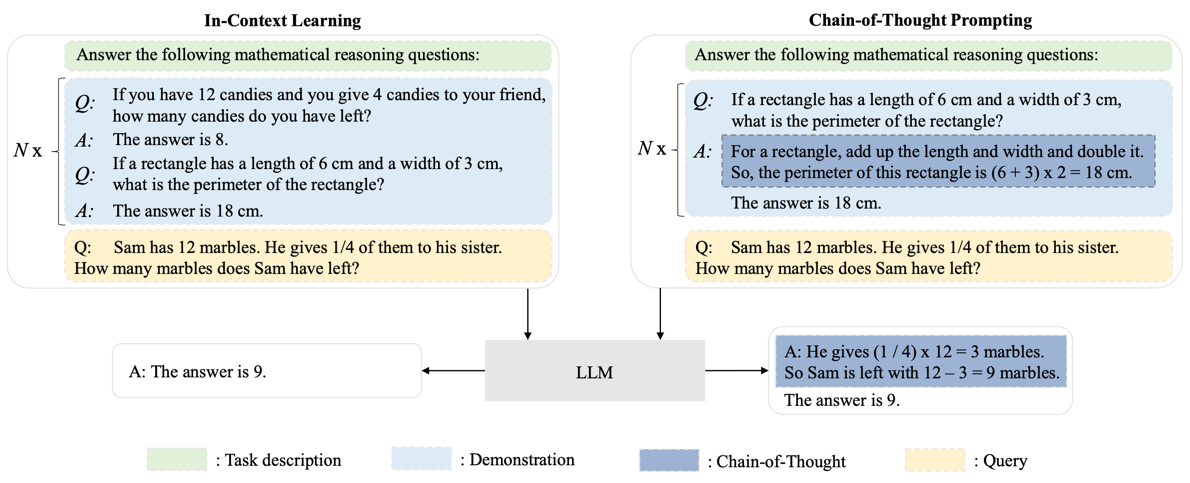
\includegraphics[width=\textwidth]{icl-vs-cot}
	\caption{A comparative illustration of in-context learning (ICL) and chain-of-thought (CoT) prompting. ICL prompts LLMs with a natural language description, several demonstrations, and a test query, while CoT prompting involves a series of intermediate reasoning steps in prompts. Source: \textcite{survey}}
	\label{fig:chain-of-thought}
\end{figure}




\section{Planning for complex tasks}
\label{sec:planning}
\lipsum